\documentclass[a4paper,12pt]{article}
\usepackage [utf8x]{inputenc}
\usepackage[czech]{babel}
\usepackage{graphicx}
\usepackage{amsmath}
\usepackage{siunitx}
\usepackage{xspace}
\usepackage{url}
\usepackage{indentfirst}
\usepackage[margin=22mm]{geometry}
\usepackage{esvect}
\usepackage{ragged2e}
\usepackage{tikz,pgf}
\usepackage{bm}
\usepackage{perpage}
\usepackage{capt-of}

\graphicspath{
	{img/}
	{plots/}
}

\newcommand{\e}{\text{e}}


\MakeSorted{figure}
\newtoks\jmenopraktika \newtoks\jmeno \newtoks\datum
\newtoks\obor \newtoks\skupina \newtoks\rocnik \newtoks\semestr
\newtoks\cisloulohy \newtoks\jmenoulohy
\newtoks\tlak \newtoks\teplota \newtoks\vlhkost
\jmenopraktika={Mikrovlnná interferometrie plazmatu}  % nahradte jmenem vaseho predmetu
\jmeno={Radek Horňák, Lukáš Vrána}            
\datum={5. 4. 2022}        % nahradte datem mereni ulohy                           
\rocnik={2.}                  
\semestr={IV.}                 
\cisloulohy={6}    % cislo ulohy           

\begin{document}
	\begin{center}
		{\Large Přírodovědecká fakulta Masarykovy univerzity} \\
		\bigskip
		{\Large \bfseries PRAKTIKUM Z~FYZIKY PLAZMATU} \\
		\bigskip
		{\Large \the\jmenopraktika}
	\end{center}
	\bigskip
	\noindent
	\setlength{\arrayrulewidth}{1pt}
	\begin{tabular*}{\textwidth}{@{\extracolsep{\fill}} l l}
		\large {\bfseries Zpracovali:}  \the\jmeno  \hspace{20mm} \large  
		{\bfseries Naměřeno:} \the\datum\\[2.5mm]
		\hline
	\end{tabular*}

\section{Teorie}
Plazma lze obecně kvalitativně považovat za vodič, dielektrikum či magnetickou kapalinu. 
Výběr modelu je závislý na konkrétní situaci. V případě interakce elektromagnetického 
záření s plazmatem se v oblasti nízkých frekvencí plazma popisuje jako vodič pomocí 
nízkofrekvenční vodivost, při vysokých frekvencích je vhodná aplikace dielektrického modelu 
včetně definice vysokofrekvenční permitivity. Hranicí mezi nízkými a vysokými frekvencemi 
je plazmová frekvence $\omega_\text{pl}$, od které se může vlna plazmatem šířit. Ta souvisí 
s hustotou plazmatu pomocí vztahu

\begin{equation}
	\omega_\text{pl} = \frac{n_\text{e} e^2}{m_\text{e} \epsilon_0}
\end{equation}
kde $n_\text{e}$ je koncentrace volných elektronů, $e$ elementární náboj, $m_\text{e}$ hmotnost 
elektronu a $\epsilon_0$ permitivita vakua.

Pro dielektrický model nemagnetického plazmatu je permitivita komplexní skalár ve tvaru $\epsilon_\text{r} = \epsilon_1 + i\epsilon_2$. V případě, 
že pro popis rozdělení rychlosti elektronů zvolíme Maxwellovo rozdělení, je relativní 
permitivita popsaná vztahem

\begin{equation}
	\epsilon_\text{r} = 1- \frac{n_\text{e} e^2 (\omega - i \nu_\text{m})}{m_\text{e} \epsilon_0 \omega (\omega^2 +\nu_\text{m}^2)}
	\label{komplexnipermitivita}
\end{equation}
kde $\nu_\text{m}$ je srážková frekvenci pro přenos hybnosti elektron--neutrál. Na rozdíl 
od běžných dielektrik je reálná část permitivity plazmatu menší než jedna. Místo relativní permitivity  můžeme obdobně popisovat plazma pomocí komplexního indexu lomu
$N = n + i\kappa$, přičemž mezi ním a relativní permitivitou je vztah $N^2$ = $\epsilon_\text{r}$. Pro jeho složky platí

\begin{equation}
	n = \sqrt{\frac{\epsilon_1 + \sqrt{\epsilon_1^2 + \epsilon_2^2}}{2}}
	\label{realna}
\end{equation}

\begin{equation}
	\kappa = \sqrt{\frac{-\epsilon_1 + \sqrt{\epsilon_1^2 + \epsilon_2^2}}{2}}
	\label{imaginarni}
\end{equation}

Reálná část indexu lomu je
přímo úměrná fázové rychlosti vlny a tedy i fázovému posuvu $\Delta\phi$. Platí vztah

\begin{equation}
 	\Delta\phi = k_0(1-n) \Delta z
 	\label{posun}
\end{equation}
kde k$_0$ je vlnové číslo a $\Delta z$ kus dráhy.  

\subsection{Stanovení koncentrace elektronů}
Pro stanovení koncentrace elektronů aproximujeme vztah pro relativní permitivitu 
\eqref{komplexnipermitivita} tak, že zanedbáme imaginární složku a vypustíme 
$\nu_\text{m}^2)$. Dostáváme

\begin{equation}
	\epsilon_\text{r} = 1- \frac{n_\text{e} e^2}{m_\text{e} \epsilon_0 \omega^2}
	\label{permitivita}
\end{equation}
Po dosazení do \eqref{posun} a úpravách můžeme vyjádřit koncentraci elektronů
v závislosti na fázovém posunu jako

\begin{equation}
	n_\text{e} = \frac{1-\left(1- \frac{\Delta\phi}{k_0 \Delta z} \right)^2
	m_\text{e} \epsilon_0 \omega^2}{e^2}
\end{equation}

\subsection{Stanovení srážkové frekvence}
Pomocí Taylorova rozvoje je možné dojít k tvaru imaginární části indexu lomu
\begin{equation}
	\kappa = \frac{|\epsilon_2|}{2\sqrt{2}|\epsilon_1|}
\end{equation}
Zkombinováním tohoto vztahu s \eqref{komplexnipermitivita}, \eqref{realna}, \eqref{imaginarni} a zanedbáním kvadratických členů můžeme vyjádřit srážkovou frekvenci jako

\begin{equation}
	\nu_\text{m} = \frac{c \ln \frac{P_0}{P} 2 \sqrt{2}|\epsilon_1|}{2\omega \Delta z \frac{n_\text{e} e^2}{m_\text{e} \epsilon_0 \omega^3}}
\end{equation}
kde $P_0$ je dodávaný výkon a $P$ je součet prošlého a odraženého výkonu.
Výpočet srážkové frekvence tedy předpokládá znalost koncentrace elektronů.

%za $\Delta z$ rozměr co zabírá výbojka ve vlnovodu
%fázový posun zjistíme z měření S21
\section{Měření a výsledky}
Měřící aparatura se skládá ze zářivky procházející vlnovodem. Uvnitř ní je
zapálený doutnavý výboj v argonu a parách rtuti 
za sníženého tlaku, typicky kolem 400 \si{\pascal}. Schéma aparatury je na obr.
\ref{schema}. Důležitým prvkem v zapojení je Vector Network Analyzer (VNA),
který zastává funkci vysokofrekvenčního zdroje i detektoru.
V klasickém interferometrickém experimentu je signál ze zdroje rozdělený do
referenční a měřící větve, které jsou nakonec svedeny dohromady. Výsledný 
detekovaný signál je tedy interferencí signálů z obou větví. Abychom kromě 
změny fáze také detekovali změnu amplitudy signálu, je potřeba použít metodu 
kvadraturní detekce se dvěma detektory. VNA, jehož schéma je vidět na 
obr. \ref{vna}, má uvnitř integrovanou referenční větev včetně detektorů, 
nám tedy stačí přes dva porty připojit měřící větev. Prostřednictvím VNA měříme $S$ parametry rozptylové matice.

\begin{figure}[h]
	\centering
	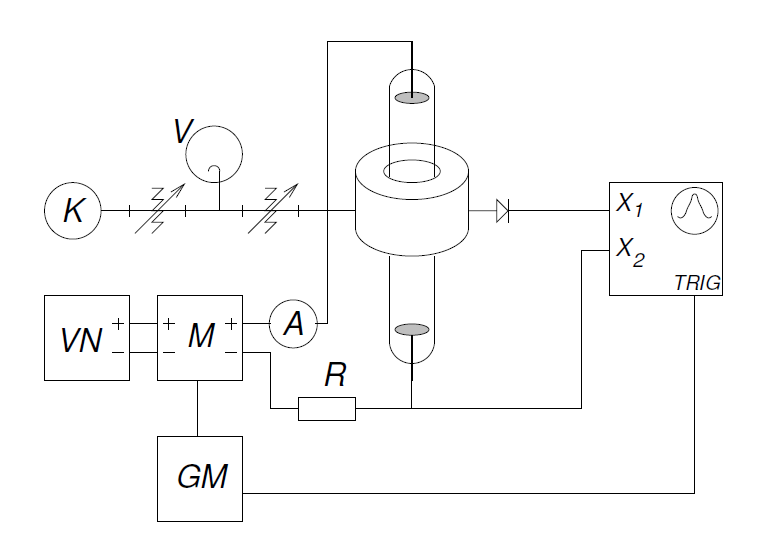
\includegraphics[width=110mm]{schema.png}
	\caption{Schéma měřící aparatury}
	\label{schema}
\end{figure}

\begin{figure}[h]
	\centering
	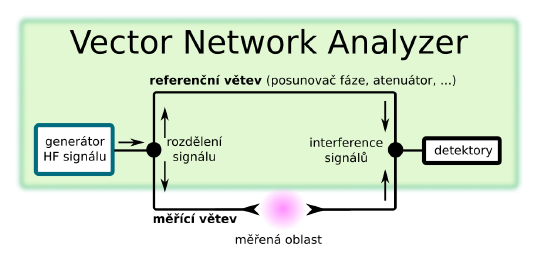
\includegraphics[width=110mm]{vna.png}
	\caption{}
	\label{vna}
\end{figure}

Před měřením je potřeba VNA zkalibrovat. To se klasicky provádí pomocí definovaných
zátěží -- short, open a match. Měření probíhá následovně: Na vysokonapěťovém zdroji
měníme proud mezi hodnotami 0,2--3 \si{\milli\ampere} a zaznamenáváme fázi a prošlý
výkon parametru $S_{21}$. Odražený výkon zanedbáváme. První sadu dat měříme pro oblast
frekvencí 1,5--3 \si{\giga\hertz}. Na VNA máme zapnuté x10 průměrování, čímž potlačíme
šum. Každé dvě měření s určitými hodnotami proudu na zářivce vystřídáme měřením s
nulovým proudem, tedy vypnutou zářivkou. Při zpracování dat poté vztahujeme jednotlivá
měření k nejbližšímu s nulovým proudem. Tímto způsobem tedy zkoumáme vliv výboje v zářivce umístěné ve vlnovodu na procházející signál vlnovodem.

Druhou sadu dat jsme naměřili stejným způsobem pro menší oblast frekvencí 2,235--2,265 \si{\giga\hertz}.

Ve výpočtech vystupuje veličina $\Delta z$, kterou jsme obecně označili jako kus dráhy.
V našem případě se jedná o tloušťku plazmatu, kterou je potřeba odhadnout. To provedeme
pomocí geometrické úvahy ze znalosti příčného rozměru vlnovodu 86 \si{\milli\meter},
průměru zářivky 18 \si{\milli\meter} a úhlu mezi zářivkou a vlnovodem 35$^{\circ}$. Za
předpokladu, že zářivka má objem válce, který následně aproximujeme pravidelným
čtyřbokým hranolem, tloušťka plazmatu podél nejdelšího rozměru vlnovodu je 24,6 \si{\milli\meter}.

\section{Závěr}


\end{document}
